\section{模块设计}
    \subsection{取指令模块}
        \subsubsection{端口说明}
                    \begin{tabularx}{\textwidth}{lll}
            \toprule
            端口名          & 端口方向  & 端口类型 \\
            \cmidrule(l){2-3}
            &
            \multicolumn{2}{X}{端口描述} \\
            \midrule
            clk             & in        & std\_logic \\
            \cmidrule(l){2-3}
            &
            \multicolumn{2}{X}{
                CPU时钟信号
            } \\
            \midrule
            state           & in        & std\_logic\_vector(3 downto 0) \\
            \cmidrule(l){2-3}
            &
            \multicolumn{2}{X}{
                CPU当前状态
            } \\
            \midrule
            PCSrc           & in        & std\_logic\_vector(31 downto 0) \\
            \cmidrule(l){2-3}
            &
            \multicolumn{2}{X}{
                说明:非异常状态下的指令地址。

                来源:WB模块。

                到达时间:当前指令InsF上升沿之前。

                产生时间:上一条指令WB上升沿之后。
            } \\
            \midrule
            EBase           & in        & std\_logic\_vector(31 downto 0) \\
            \cmidrule(l){2-3}
            &
            \multicolumn{2}{X}{
                说明:异常处理基地址。

                来源:CP0模块。

                到达时间:当前指令InsF上升沿到来之前。
            } \\
            \midrule
            EPC             & in        & std\_logic\_vector(31 downto 0) \\
            \cmidrule(l){2-3}
            &
            \multicolumn{2}{X}{
                说明:ERET指令的返回地址。

                来源:CP0模块。

                到达时间:当前指令InsF上升沿到来之前。
            } \\
            \midrule
            pc\_sel         & in        & std\_logic\_vector(1 downto 0) \\
            \cmidrule(l){2-3}
            &
            \multicolumn{2}{X}{
                pc\_sel(1):

                    说明:eret\_enable,使能信号。

                    来源:ID模块。

                    到达时间:当前指令InsF上升沿到来之前。

                    产生时间:上一条指令ID上升沿之后。
                    
                pc\_sel(0):

                    说明:pc\_control,判断是否为异常状态。

                    来源:异常模块。

                    到达时间:当前指令InsF上升沿到来之前。
            } \\
            \midrule
            PC              & out       & std\_logic\_vector(31 downto 0) \\
            \cmidrule(l){2-3}
            &
            \multicolumn{2}{X}{
                说明:PC寄存器,时序逻辑。

                产生时间:当前指令InsF上升沿到来之后。

                有效时间:直到下一条指令的IF阶段。
            } \\
            \midrule
            PCmmu           & out       & std\_logic\_vector(31 downto 0) \\
            \cmidrule(l){2-3}
            &
            \multicolumn{2}{X}{
                说明:为MMU单元提供的PC,组合逻辑。

                产生时间:当前指令InsF上升沿到来之前。

                有效时间:直到当前指令IF阶段结束。
            } \\
            \bottomrule
            \end{tabularx}
 

            \begin{figure}[!hbp]
                \centering
                \caption{取指令模块端口示意图}
                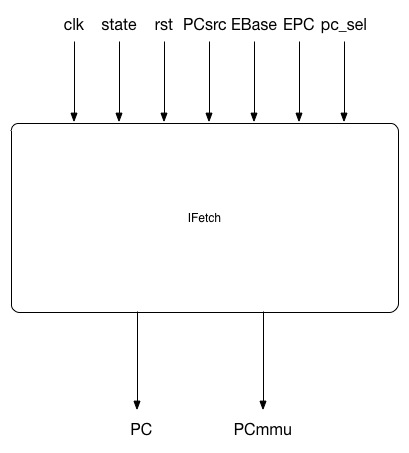
\includegraphics[width=0.5\textwidth]{chart/ifetch.jpg}
            \end{figure}
        \subsubsection{内部实现}
            需要的数据有PcSrc、EBase、EPC。

            PcSrc产生于上一条指令的WB阶段。%
            EBase为固定值,直接从CP0部分连接过来。%
            EPC在异常阶段写入,直接从CP0部分连接过来。%
            pc\_sel为上一条指令的解码阶段产生。%
            因此,所有的数据都能够在InsF时钟上升沿之前准备完毕。

            内部分为两个部分对PC进行计算:%
            首先为组合逻辑部分,需要在InsF时钟上升沿到来之前为MMU计算出PC值,%
            因此建立一个process,敏感信号为全部的PC选择信息,%
            即时计算出PC值,连接到MMU部分,%
            使得MMU能够在InsF上升沿进行取指令的操作。%
            其次为时序逻辑部分,在InsF时钟上升沿时,%
            对PC进行选择,选择方式与PCmmu相同。%
            此process产生的PC,在当前指令的全部周期有效,%
            是计算RPC、branch、jump的地址的基础。%
    \subsection{指令解析模块}
        \subsubsection{端口说明}
                    \begin{tabularx}{\textwidth}{lll}
            \toprule
            端口名          & 端口方向  & 端口类型 \\
            \cmidrule(l){2-3}
            &
            \multicolumn{2}{X}{端口描述} \\
            \midrule
            clk             & in        & std\_logic \\
            \cmidrule(l){2-3}
            &
            \multicolumn{2}{X}{
                CPU时钟信号。
            } \\
            \midrule
            rst             & in        & std\_logic \\
            \cmidrule(l){2-3}
            &
            \multicolumn{2}{X}{
                初始化信号,在CPU启动时使用。
            } \\
            \midrule
            state           & in        & status(自定义状态集合) \\
            \cmidrule(l){2-3}
            &
            \multicolumn{2}{X}{
                CPU当前状态。
            } \\
            \midrule
            instruction     & in        & std\_logic\_vector(31 downto 0) \\
            \cmidrule(l){2-3}
            &
            \multicolumn{2}{X}{
                说明:当前指令。

                来源:MMU模块。

                到达时间:当前指令InsD上升沿之前。

                产生时间:当前指令InsF上升沿之后。
            } \\
            \midrule
            instr\_out      & out       & std\_logic\_vector(31 downto 0) \\
            \cmidrule(l){2-3}
            &
            \multicolumn{2}{X}{
                说明:指令寄存器,除三个寄存器的编号,%
                其他所有控制线均从此产生。%
                之后周期中如果需要用到指令也从此处获得。

                产生时间:当前指令InsD上升沿之后。
            } \\
            \midrule
            rs\_addr        & out       & std\_logic\_vector(4 downto 0) \\
            \cmidrule(l){2-3}
            &
            \multicolumn{2}{X}{
                说明:通用寄存器编号1,在InsD阶段需要读取到值。

                产生时间:当前指令InsD上升沿之前。
            } \\
            \midrule
            rt\_addr        & out       & std\_logic\_vector(4 downto 0) \\
            \cmidrule(l){2-3}
            &
            \multicolumn{2}{X}{
                说明:通用寄存器编号2、写入寄存器编号,在InsD阶段需要读取到值。

                产生时间:当前指令InsD上升沿之前。
            } \\
            \midrule
            rd\_addr        & out       & std\_logic\_vector(4 downto 0) \\
            \cmidrule(l){2-3}
            &
            \multicolumn{2}{X}{
                说明:CP0寄存器编号、写入寄存器编号,在InsD阶段需要读取到值。

                产生时间:当前指令InsD上升沿之前。
            } \\
            \midrule
            pc\_op          & out       & std\_logic\_vector(1 downto 0) \\
            \cmidrule(l){2-3}
            &
            \multicolumn{2}{X}{
                说明:PCSrc选择器,正常状态下PC的选择方式。%
                输出到WB模块,4选1数据选择器的控制信号,选择正确的PC。

                产生时间:当前指令InsD上升沿之后。

                有效时间:下一条指令InsD上升沿之后。 
            } \\
            &
            \multicolumn{2}{X}{
                00 PC+4的计算结果。

                01 branch指令PC计算的结果。

                10 jump指令目标地址。

                11 主ALUOut计算结果。
            } \\
            \midrule
            eret\_enable    & out       & std\_logic \\

            \cmidrule(l){2-3}
            &
            \multicolumn{2}{X}{
                说明:ERET使能,对PC进行选择。%
                专门对ERET指令使用,输出到IFetch模块。

                产生时间:当前指令InsD上升沿之后。

                有效时间:下一条指令InsD上升沿之后。 
            } \\
            \midrule
            comp\_op        & out       & std\_logic\_vector(2 downto 0) \\
            \cmidrule(l){2-3}
            &
            \multicolumn{2}{X}{
                说明:比较信号,branch指令的跳转条件。%
                输出到WB模块,如果为branch系列指令则通过此信号进行选择。

                产生时间:当前指令InsD上升沿之后。

                有效时间:下一条指令InsD上升沿之后。 
            } \\
            &
            \multicolumn{2}{X}{
                000 BEQ(R[s] = R[t])

                001 BGEZ(R[s] >= 0)

                010 BGTZ(R[s] > 0)
            } \\
            &
            \multicolumn{2}{X}{
                011 BLEZ(R[s] <= 0)

                100 BLTZ(R[s] < 0)

                101 BNE(R[s] != R[t])
            } \\
            \midrule
            imme            & out       & std\_logic\_vector(31 downto 0) \\
            \cmidrule(l){2-3}
            &
            \multicolumn{2}{X}{
                说明:32位立即数,针对不同指令的需求产生。%
                立即数本身作为ALUSrc的来源之一。

                产生时间:当前指令InsD上升沿之后。

                有效时间:下一条指令InsD上升沿之后。 
            } \\
            &
            \multicolumn{2}{X}{
                立即数产生方式有四种,均为从不同立即数长度扩展为32位。

                16位有符号扩展,16位无符号扩展,%
                移位指令需要的5位到32位扩展,jump指令的立即数扩展。
            } \\
            \midrule
            alu\_ops        & out       & std\_logic\_vector(8 downto 0) \\
            \cmidrule(l){2-3}
            &
            \multicolumn{2}{X}{
                说明:控制ALU模块。

                ALUSrcA(8 downto 7):ALU第一输入的选择信号,%
                四选一数据选择。

                ALUSrcB(6 downto 5):ALU第二输入的选择信号,%
                四选一数据选择。
            } \\
            &
            \multicolumn{2}{X}{
                ALUOp(4 downto 0):ALU操作,%
                5位,整合了乘法器相关运算,详细说明见ALU模块说明。

                产生时间:当前指令InsD上升沿之后。

                有效时间:下一条指令InsD上升沿之后。 
            } \\
            \midrule
            mem\_op         & out       & std\_logic\_vector(2 downto 0) \\
            \cmidrule(l){2-3}
            &
            \multicolumn{2}{X}{
                说明:控制MEM模块。

                MEMRead(2):是否可读内存。

                MEMWrite(1):是否可写内存。

                MEMValue(0):选择写入内存的值,%
                寄存器的数据或者SB指令处理之后的数据。
            } \\
            &
            \multicolumn{2}{X}{
                产生时间:当前指令InsD上升沿之后。

                有效时间:下一条指令InsD上升沿之后。
            } \\
            \midrule
            wb\_op          & out       & std\_logic\_vector(4 downto 0) \\
            \cmidrule(l){2-3}
            &
            \multicolumn{2}{X}{
                说明:控制WB模块。

                产生时间:当前指令InsD上升沿之后。

                有效时间:下一条指令InsD上升沿之后。 
            } \\
            &
            \multicolumn{2}{X}{
                RegDst(5 downto 4):写回寄存器编号。
                如果为00则写回16到20位rt寄存器,%
                如果为01则写回11到15位rd寄存器,%
                如果为10则写回31号寄存器。
                如果为11则不写寄存器。
            } \\
            &
            \multicolumn{2}{X}{
                RegValue(3 downto 1):写回寄存器的内容%

                000 主ALU计算结果

                001 读取内存的数据

                010 RPC
            } \\
            &
            \multicolumn{2}{X}{
                011 Zero-extend内存byte

                100 Signed-extend内存byte

                101 Zero-extend内存word

                110 CP0寄存器
            } \\
            \midrule
            cp0\_op         & out       & std\_logic\_vector(1 downto 0) \\
            \cmidrule(l){2-3}
            &
            \multicolumn{2}{X}{
                说明:控制CP0模块。

                EPCValue(1):异常产生时,EPC写入的内容,%
                选择写入PC或者PC+4。

                CP0Write(0):CP0寄存器是否可写。
            } \\
            &
            \multicolumn{2}{X}{
                产生时间:当前指令InsD上升沿之后。

                有效时间:下一条指令InsD上升沿之后 
            } \\
            \midrule
            tlbwi\_enable   & out       & std\_logic \\
            \cmidrule(l){2-3}
            &
            \multicolumn{2}{X}{
                说明:TLB写使能。

                产生时间:当前指令InsD上升沿之后。

                有效时间:下一条指令InsD上升沿之后。
            } \\
            \midrule
            exc\_code   & out       & std\_logic\_vector(1 downto 0) \\
            \cmidrule(l){2-3}
            &
            \multicolumn{2}{X}{
                说明:指令解析模块产生的异常

                产生时间:当前指令InsD下降沿之后,在下一条指令的下降沿时消除

                有效时间:一个CPU时钟周期,需要异常模块及时处理。
            } \\
            &
            \multicolumn{2}{X}{
                00 没有产生异常

                01 syscall

                10 未定义的指令异常
            } \\
            \bottomrule
            \end{tabularx}

            \begin{figure}[!hbp]
                \centering
                \caption{指令解析模块端口示意图}
                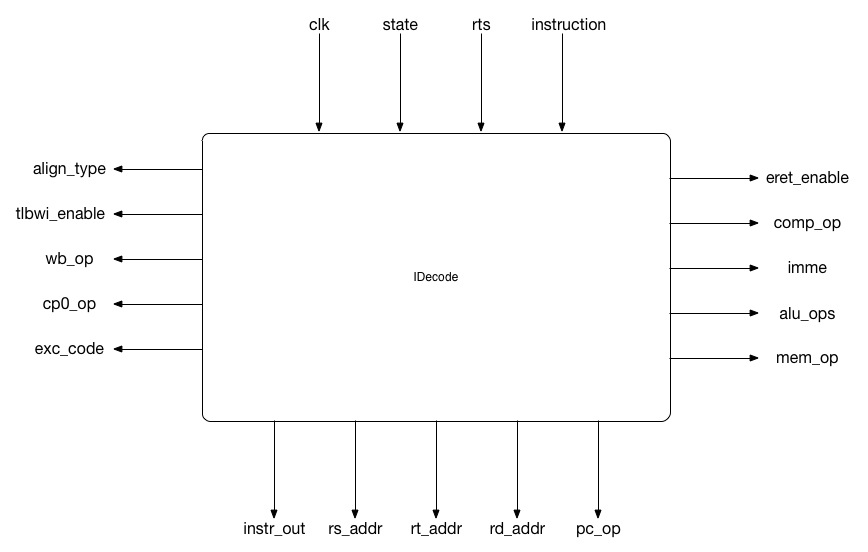
\includegraphics[width=0.9\textwidth]{chart/idecode.jpg}
            \end{figure}

        \subsubsection{内部实现}
            需要的数据有instruction,%
            产生于当前指令InsF上升沿之后,能够在当前指令InsD上升沿之前到达。

            内部实现分为两部分:%
            \begin{enumerate}
            \item
            在InsD阶段除了解码指令之外,%
            还需要读取通用寄存器和CP0寄存器的值。%
            需要在InsD上升沿到来之前,将三个寄存器编号发送给寄存器堆。%
            因此将instruction的三个5位的寄存器编号直接连接到输出的rs、rt、rd部分。%
            \item
            其他控制线的生成均通过时钟驱动,%
            在IDEcode有相应寄存器,连接至输出端。%
            在InsD时钟上升沿之后,根据指令解码产生控制信号。%
            产生的控制信号根据需要,%
            输出到ALU、WB、MEM、CP0、IFetch、MMU模块。
            \item
            异常:

            在指令解码阶段可能产生两种异常:系统调用或者未定义的指令异常。%
            由于ALUOp的生成需要使用case语句对每条指令单独处理,%
            因此选择在case的when others部分生成未定义的指令异常%
            如果是syscall则产生异常,并且将ALUOp置为无用的操作。%

            异常信号产生的时间为指令解码阶段的时钟下降沿,%
            直接通过exc\_code输出到异常处理模块,再利用其控制CPU主状态机的工作流程。

            异常在下一个时钟的下降沿会被消除,因此需要异常处理模块即使将异常信息捕获。

            \end{enumerate}

    \subsection{ALU模块}
        \subsubsection{端口说明}
                    \begin{tabularx}{\textwidth}{lll}
            \toprule
            端口名          & 端口方向 & 端口类型 \\
            \cmidrule(l){2-3}
                            & \multicolumn{2}{l}{端口描述} \\
            \midrule
            clk             & in       & std\_logic \\
            \cmidrule(l){2-3}
            &
            \multicolumn{2}{X}{CPU时钟信号。} \\
            \midrule
            enable          & in       & std\_logic \\
            \cmidrule(l){2-3}
            & 
            \multicolumn{2}{X}{
            ALU模块是否使能,为1时工作,为0时不工作,%
            需要在clk时钟上升沿之前准备好,%
            并保持到clk时钟上升沿之后一极短时间。} \\
            \midrule
            rs\_value        & in       & std\_logic\_vector(31 downto 0) \\
            \cmidrule(l){2-3}
            &
            \multicolumn{2}{X}{
            来自通用寄存器堆的第一个值。需要在clk时钟上升沿之前准备好,%
            并保持到clk时钟上升沿之后一极短时间。} \\
            \midrule
            rt\_value        & in       & std\_logic\_vector(31 downto 0) \\
            \cmidrule(l){2-3}
            & 
            \multicolumn{2}{X}{
            来自通用寄存器堆的第二个值。需要在clk时钟上升沿之前准备好,%
            并保持到clk时钟上升沿之后一极短时间。} \\
            \midrule
            imme            & in       & std\_logic\_vector(31 downto 0) \\
            \cmidrule(l){2-3}
            &
            \multicolumn{2}{X}{
            指令中包含的立即数,来自指令解析模块。%
            需要在clk时钟上升沿之前准备好,%
            并保持到clk时钟上升沿之后一极短时间。} \\
            \midrule
            cp0\_value      & in       & std\_logic\_vector(31 downto 0) \\
            \cmidrule(l){2-3}
            &
            \multicolumn{2}{X}{
            来自cp0寄存器,mfc0指令需要。%
            需要在clk时钟上升沿之前准备好,%
            并保持到clk时钟上升沿之后一极短时间。} \\
            \midrule
            state           & in       & std\_logic\_vector(3 downto 0) \\
            \cmidrule(l){2-3}
            &
            \multicolumn{2}{X}{
            来自状态控制模块,用来指示当前处于工作状态的模块。%
            若当前非ALU工作状态,%
            则任何外部输入都不会对ALU的hi、lo寄存器以及ALU的输出造成修改。%
            需要在clk时钟上升沿之前准备好,%
            并保持到clk时钟上升沿之后一极短时间。} \\
            \midrule
            alu\_op         & in       & std\_logic\_vector(4 downto 0) \\
            \cmidrule(l){2-3}
            &
            \multicolumn{2}{X}{
            来自指令解析模块的ALU运算操作符。%
            需要在clk时钟上升沿之前准备好,%
            并保持到clk时钟上升沿之后一极短时间。%
            各操作符代表的意义为%
            (A、B分别代表经过alu\_srcA、alu\_srcB选择后的值,%
            result代表alu\_result,lo、hi代表乘法寄存器):%
            } \\
            &
            \multicolumn{2}{X}{
            00000 result = A + B

            00001 result = A - B

            00010 result = A - B(比较大小,实际做减法)

            00011 result = A \& B
            } \\
            &
            \multicolumn{2}{X}{
            00100 result = A | B

            00101 result = A \textasciicircum \ B

            00110 result = ~(A | B)

            00111 result = B << A
            } \\
            &
            \multicolumn{2}{X}{
            01000 result = B >> A(算术右移)

            01001 result = B >> A(逻辑右移)
            } \\
            &
            \multicolumn{2}{X}{
            01010 result = A < B?(有符号比较,结果真时最低位输出1,否则输出0,其他位总是输出0)

            01011 result = A < B?(无符号比较,结果真时最低位输出1,否则输出0,其他位总是输出0)
            } \\
            &
            \multicolumn{2}{X}{
            10000 hi\_lo = A * B(补码乘法)

            10001 result = lo

            10010 result = hi
            } \\
            &
            \multicolumn{2}{X}{
            10011 lo = A

            10100 hi = A} \\
            \midrule
            alu\_srcA & in & std\_logic\_vector(1 downto 0) \\
            \cmidrule(l){2-3}
            &
            \multicolumn{2}{X}{
            ALU的第一个操作数的选择码,%
            当值为“00”时选取rs\_value,%
            当值为“01”时选取imme,当值为“10”时选取cp0\_value,%
            当值为“11”时选取立即数16。需要在clk时钟上升沿之前准备好,%
            并保持到clk时钟上升沿之后一极短时间。
            } \\
            \midrule
            alu\_srcB & in & std\_logic\_vector(1 downto 0) \\
            \cmidrule(l){2-3}
            &
            \multicolumn{2}{X}{
            ALU的第二个操作数的选择码,当值为“00”时选取rt\_value,%
            当值为“01”时选取imme,当值为“10”时选取cp0\_value。%
            需要在clk时钟上升沿之前准备好,%
            并保持到clk时钟上升沿之后一极短时间。
            } \\
            \midrule
            alu\_result & out & std\_logic\_vector(31 downto 0) \\
            \cmidrule(l){2-3}
            &
            \multicolumn{2}{X}{
            ALU的输出,在下一个时钟上升沿之前准备好,%
            并保持直到下一次能使ALU输出改变%
            (state为ALU工作状态、enable为1、alu\_op非写hi、lo寄存器)%
            的时钟上升沿。
            } \\
            \bottomrule
            \end{tabularx}

            \begin{figure}[!hbp]
                \centering
                \caption{ALU模块端口示意图}
                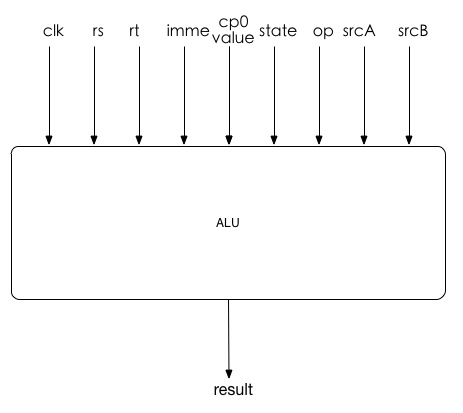
\includegraphics[width=0.7\textwidth]{chart/alu.jpg}
            \end{figure}

        \subsubsection{内部实现}
            每次时钟上升沿到来时,检查state,%
            若不是ALU工作状态则不进行任何操作。%
            根据alu\_srcA选择第一个操作数,根据alu\_srcB选择第二个操作数,%
            根据操作码进行相应的运算,将结果输出或保存到hi、lo寄存器中。

            注意乘法运算需要较多的时间,因此若在某一个时钟上升沿进行乘法运算,%
            不能认为在下一个时钟上升沿就能在hi、lo寄存器中取到正确的结果。%
            一般来说,在25MHz时钟频率下进行乘法运算在1个时钟周期内可以完成,%
            那么如果在此频率运行的CPU上,%
            可以保证两条连续的乘法、取hi(lo)寄存器指令能得到正确的结果。%
            乘法运算时间需要根据不同的硬件平台、时钟频率进行测量,%
            不能一概而论。
    \subsection{访存模块}
        \subsubsection{端口说明}
                    \begin{tabularx}{\textwidth}{lll}
            \toprule
            端口名      & 端口方向  & 端口类型 \\
            \cmidrule(l){2-3}
            &
            \multicolumn{2}{X}{端口描述} \\
            \midrule
            result      & in   & std\_logic\_vector(31 downto 0) \\
            \cmidrule(l){2-3}
            &
            \multicolumn{2}{X}{
                说明:访存地址

                来源:ALU模块

                到达时间:指令执行阶段时钟上升沿后。

                保持时间:至少保持到访存阶段时钟上升沿之后。
            } \\
            \midrule
            mem\_op      & in    & std\_logic\_vector(2 downto 0) \\
            \cmidrule(l){2-3}
            &
            \multicolumn{2}{X}{
                说明:内存操作控制线

                来源:IDecode模块
                
                到达时间:指令解码时钟上升沿之后。

                保持时间:至少保持到访存阶段结束。
            } \\
            &
            \multicolumn{2}{X}{
                mem\_op(2): memRead:内存读使能。

                mem\_op(1): memWrite:内存写使能。

                mem\_op(0): memValue:内存写入数据。
                如果为0则写入来自寄存器的数据,%
                如果为1则写入SB指令处理之后的数据。
            } \\
            \midrule
            rt\_value   & in    & std\_logic\_vector(31 downto 0) \\
            \cmidrule(l){2-3}
            &
            \multicolumn{2}{X}{
                说明:来自寄存器的数值,访存阶段写入数据的可能来源之一。

                来源:通用寄存器。

                到达时间:指令解码时钟上升沿之后。
            } \\
            \midrule
            mmu\_value  & in    & std\_logic\_vector(31 downto 0) \\
            \cmidrule(l){2-3}
            &
            \multicolumn{2}{X}{
                说明:访存得到的数据,为SB指令提供支持。

                来源:MMU模块。

                到达时间:第二次访存操作上升沿之前。

                产生时间:第一次访存操作下降沿之后。
            } \\
            \midrule
            addr\_mmu    & out  & std\_logic\_vector(31 downto 0) \\
            \cmidrule(l){2-3}
            &
            \multicolumn{2}{X}{
                说明:访存阶段的地址。

                产生时间:访存阶段时钟上升沿之前。
            } \\
            \midrule
            write\_value & out & std\_logic\_vector(31 downto 0) \\
            \cmidrule(l){2-3}
            &
            \multicolumn{2}{X}{
                说明:访存阶段写入数据。

                产生时间:访存阶段时钟上升沿之前。
            } \\
            \midrule
            read\_enable & out & std\_logic \\
            \cmidrule(l){2-3}
            &
            \multicolumn{2}{X}{
                说明:访存读使能。
            } \\
            \midrule
            write\_enable & out & std\_logic \\
            \cmidrule(l){2-3}
            &
            \multicolumn{2}{X}{
                说明:访存写使能。
            } \\
            \bottomrule
        \end{tabularx}

            \begin{figure}[!hbp]
                \centering
                \caption{访存模块端口示意图}
                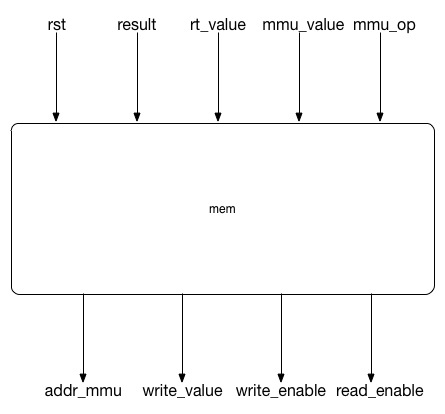
\includegraphics[width=0.6\textwidth]{chart/mem.jpg}
            \end{figure}

        \subsubsection{内部实现}
            \begin{enumerate}
            \item
            MEM模块在指令的执行周期之后,%
            但是内存访问模块需要使用访存周期的时钟上升沿,%
            因此MEM模块不能占用时钟上升沿,%
            需要设计为一个组合逻辑模块。%
            其主要功能为访存周期的预处理,%
            为其生成访存的地址与写入的数据,以及产生使能信号。
            \item
            MEM模块内部完全由组合逻辑实现。%

            目前MEM模块有一些输入输出之间采取的是直接连线的方式,%
            主要目的在于比较清晰地体现出访存的设计思路。%
            后期可能将部分连线直接连接到MMU模块,%
            或者在Xilinx编译与优化的过程中,由编译器直接优化掉。

            直接连线部分:%
            addr\_mmu输出直接与输入的result端口相连,%
            将访存地址直接输出到MMU模块。%
            read\_enable输出直接与输入的mem\_op(2)相连,%
            将读使能输出到MMU模块。%
            write\_enable输出直接与输入的mem\_op(1)相连,
            将写使能输出到MMU模块。
        
            组合逻辑部分:%
            wrirte\_value为内存写入值,需要根据memValue信号进行选择。%
            如果memValue为0,则write\_value的取值为rt\_value,%
            写入寄存器2的值。%
            如果memValue为1,说明此条指令为SB指令,有两个访存阶段。%
            第一访存阶段为读,此时不需要write\_value的值。%
            第二访存阶段为写,%
            在此阶段开始之前,%
            第一访存阶段已经取出内存中addr\_mmu地址中的数据,%
            在此基础上进行一个byte的修改,%
            利用addr\_mmu最后两位选择修改位置,%
            将rt\_value的最低位byte写入,%
            整体作为内存的写入值传递给MMU模块。%
        \end{enumerate}
    \subsection{写回模块}
        \subsubsection{端口说明}
                    \begin{tabularx}{\textwidth}{lll}
            \toprule
            端口名          & 端口方向  & 端口类型 \\
            \cmidrule(l){2-3}
            &
            \multicolumn{2}{X}{端口描述} \\
            \midrule
            clk             & in        & std\_logic \\
            \cmidrule(l){2-3}
            &
            \multicolumn{2}{X}{
                CPU时钟信号
            } \\
            \midrule
            state           & in        & status(自定义状态集合) \\
            \cmidrule(l){2-3}
            &
            \multicolumn{2}{X}{
                CPU当前状态
            } \\
            WB\_e           & in        & std\_logic \\
            \cmidrule(l){2-3}
            &
            \multicolumn{2}{X}{
                WB文件的使能信号
            } \\
            \midrule
            RPC             & in        & std\_logic\_vector(31 downto 0) \\
            \cmidrule(l){2-3}
            &
            \multicolumn{2}{X}{
                即本周期的PC+4,要求ALU阶段上升沿之前准备好。
            } \\
            \midrule
            mmu\_value      & in        & std\_logic\_vector(31 downto 0) \\
            \cmidrule(l){2-3}
            &
            \multicolumn{2}{X}{
                来自MMU的读取值,要求WB阶段上升沿之前准备好。
            } \\
            \midrule
            cp0\_value      & in        & std\_logic\_vector(31 downto 0) \\
            \cmidrule(l){2-3}
            &
            \multicolumn{2}{X}{
                来自CP0的读取值,要求WB阶段上升沿之前准备好。
            } \\
            \midrule
            alu\_result     & in        & std\_logic\_vector(31 downto 0) \\
            \cmidrule(l){2-3}
            &
            \multicolumn{2}{X}{
                来自ALU的读取值,要求WB阶段上升沿之前准备好。
            } \\
            \midrule
            wb\_op          & in        & std\_logic\_vector(5 downto 0) \\
            \cmidrule(l){2-3}
            &
            \multicolumn{2}{X}{
                WB阶段写入寄存器编号的来源与写入数据的来源选择,%
                要求WB阶段上升沿之前准备好。

                4-3位为写入寄存器编号来源的控制信号:

                    00表示写入rt寄存器;

                    01表示写入rd寄存器;

                    10表示写入31寄存器;

                    11或其他信号表示不写;
            } \\
            &
            \multicolumn{2}{X}{
                2-0位为写入数据来源的控制信号:

                    000表示数据来自ALU;

                    001表示数据来自MMU;

                    010表示数据来自RPC;

                    011表示数据来自MMU,此时为LBU操作,%
                    根据alu\_result的低2位决定使用MMU数据的哪一字节,高位零扩展;
            } \\
            &
            \multicolumn{2}{X}{
                    100表示数据来自MMU,此时为LB操作,%
                    根据alu\_result的低2位决定使用MMU数据的哪一字节,高位符号扩展;

                    101表示数据来自MMU,此时为LHU操作,%
                    根据alu\_result的低2位决定使用MMU数据的哪一字节,高位零扩展;

                    110表示数据来自CP0寄存器;
            } \\
            \midrule
            rd\_addr        & in    & std\_logic\_vector(4 downto 0) \\
            \cmidrule(l){2-3}
            &
            \multicolumn{2}{X}{
                Rd寄存器编号,要求WB阶段上升沿之前准备好。
            } \\
            \midrule
            rt\_addr        & in    & std\_logic\_vector(4 downto 0) \\
            \cmidrule(l){2-3}
            &
            \multicolumn{2}{X}{
                Rt寄存器编号,要求WB阶段上升沿之前准备好。
            } \\
            \midrule
            write\_addr     & out   & std\_logic\_vector(4 downto 0) \\
            \cmidrule(l){2-3}
            &
            \multicolumn{2}{X}{
                写入通用寄存器组的地址,请在每一时钟上升沿使用。%
                保持到下一WB阶段时钟上升沿。

                对于IP core的片内RAM模块组成的通用寄存器组,%
                以下三个信号请直接接至通用寄存器组。
            } \\
            \midrule
            write\_value    & out   & std\_logic\_vector(31 downto 0) \\
            \cmidrule(l){2-3}
            &
            \multicolumn{2}{X}{
                写入通用寄存器组的数据,请在每一时钟上升沿使用。%
                保持到下一WB阶段时钟上升沿。

                对于IP core的片内RAM模块组成的通用寄存器组,%
                以下三个信号请直接接至通用寄存器组。
            } \\
            \midrule
            write\_enable   & out   & std\_logic \\
            \cmidrule(l){2-3}
            &
            \multicolumn{2}{X}{
                写入通用寄存器组的使能,请在每一时钟上升沿使用。%
                保持到下一WB阶段时钟上升沿。

                对于IP core的片内RAM模块组成的通用寄存器组,%
                以下三个信号请直接接至通用寄存器组。
            } \\
            \midrule
	        pc\_op          & in    & std\_logic\_vector(2 downto 0) \\
            \cmidrule(l){2-3}
            &
            \multicolumn{2}{X}{
                非ERET指令时,选择新PC的控制信号                                             

                    00时,选PC+4,即RPC;                                                    

                    01时,根据比较是否成立进行选择,%
                    成立则跳转到PC+4+immediate,即RPC;否则跳转到RPC。
            } \\
            &
            \multicolumn{2}{X}{
                    !!!!!!!PC+4+immediate是否已交给ALU计算。

                    10时,跳转到immediate,对应某些jump语句;

                    11时,跳转到ALU的计算结果,对应某些jump语句;

                要求WB阶段上升沿之前准备好。
            } \\
            \midrule
            comp\_op        & in    & std\_logic\_vector(2 downto 0) \\
            \cmidrule(l){2-3}
            &
            \multicolumn{2}{X}{
                比较跳转时的比较控制信号,一般对应B系列指令。跳转条件如下:

                    000时,条件为Rs的值等于Rt的值;

                    001时,条件为Rs的值>=0;

                    010时,条件为Rs的值>0;
            } \\
            &
            \multicolumn{2}{X}{
                    011时,条件为Rs的值<=0;

                    100时,条件为Rs的值<0;

                    101时,条件为Rs的值不等于Rt的值;

                    其他情况,恒为非;

                要求ALU阶段上升沿之前准备好。
            } \\
            \midrule
            rs\_value       & in    & std\_logic\_vector(31 downto 0) \\
            \cmidrule(l){2-3}
            &
            \multicolumn{2}{X}{
                Rs的值,要求ALU阶段上升沿之前准备好。
            } \\
            \midrule
            rt\_value       & in    & std\_logic\_vector(31 downto 0) \\
            \cmidrule(l){2-3}
            &
            \multicolumn{2}{X}{
                Rt的值,要求ALU阶段上升沿之前准备好。
            } \\
            \midrule
            imme            & in    & std\_logic\_vector(31 downto 0) \\
            \cmidrule(l){2-3}
            &
            \multicolumn{2}{X}{
                指令中包含的立即数,要求WB阶段上升沿之前准备好。
            } \\
            \midrule
            PcSrc            & out   & std\_logic\_vector(31 downto 0) \\
            \cmidrule(l){2-3}
            &
            \multicolumn{2}{X}{
                非ERET指令时,新PC值。                                                       
                WB阶段上升沿之后可读。
            } \\
                

            \bottomrule
        \end{tabularx}

            \begin{figure}[!hbp]
                \centering
                \caption{写回模块端口示意图}
                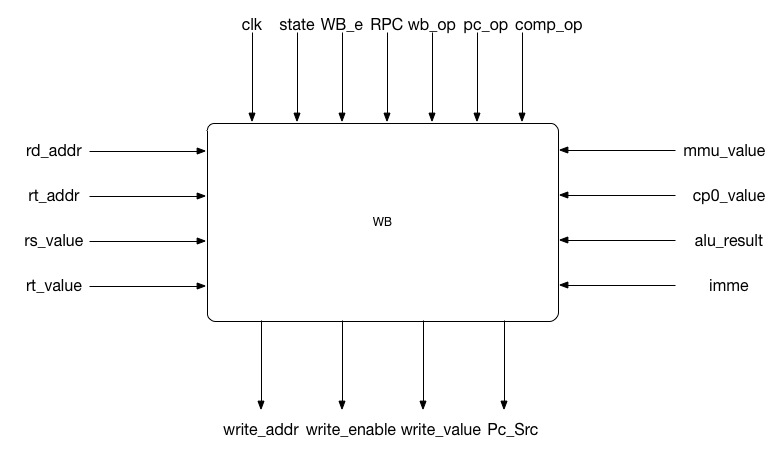
\includegraphics[width=0.9\textwidth]{chart/wb.jpg}
            \end{figure}
        \subsubsection{内部实现}
            WB文件包含两个模块,即WB模块与PC模块。%
            WB模块在WB阶段上升沿运行。%
            根据输入的控制信号,选择是否写入以及写入的寄存器编号的来源。%
            同时,根据输入的控制信号,选择从哪里获得写入数据。%
            非扩展的情况比较简单,直接将写出数据赋为相应输入值即可。%
            对于扩展的情况,%
            需要根据alu\_result选择使用mmu\_value的哪一部分作为写入数据的低位。
            对于符号扩展的情况,%
            扩展方法是根据有效位最高位决定扩展位写全0或写全1。
            
            PC模块在ALU阶段上升沿进行比较。比较方式使用compare\_op控制;%
            在WB阶段,根据pc\_op控制对输出PC的赋值。%
            其中,如果输出PC需要由比较结果决定,%
            使用ALU阶段的比较结果控制输出PC的值。%
            这一步输出的PC还需在之后使用别的控制信号决定是否用于IF。

            WB模块状态跳转:%
	        ALU阶段由ALU模块处理。%
	        WB阶段,无条件跳转至IF阶段。

            WB模块异常触发:%
	        无。

    \subsection{MMU模块}
        \subsubsection{端口说明}
                    \begin{tabularx}{\textwidth}{lll}
            \toprule
            端口名          & 端口方向  & 端口类型 \\
            \cmidrule(l){2-3}
            &
            \multicolumn{2}{X}{端口描述} \\
            \midrule
            clk             & in        & std\_logic \\
            \cmidrule(l){2-3}
            &
            \multicolumn{2}{X}{
                CPU时钟信号
            } \\
            \midrule
            state           & in        & std\_logic\_vector(3 downto 0) \\
            \cmidrule(l){2-3}
            &
            \multicolumn{2}{X}{
                说明:CPU状态机信号
            } \\
            \midrule
            if\_addr        & in        & std\_logic\_vector(31 downto 0) \\
            \cmidrule(l){2-3}
            &
            \multicolumn{2}{X}{
                说明:取指令地址

                来源:IFetch模块

                到达时间:取指令时钟上升沿之前
            } \\
            \midrule
            instruction        & out        & std\_logic\_vector(31 downto 0) \\
            \cmidrule(l){2-3}
            &
            \multicolumn{2}{X}{
                说明:取指令阶段得到的32位指令

                产生时间:访存阶段结束之后,根据ready位进行判断
            } \\
            \midrule
            virtual\_addr & in      & std\_logic\_vector(31 downto 0) \\
            \cmidrule(l){2-3}
            &
            \multicolumn{2}{X}{
                说明:访存阶段的虚拟地址

                来源:MEM模块

                到达时间:访存阶段时钟上升沿之前
            } \\
            \midrule
            data\_in & in     & std\_logic\_vector(31 downto 0) \\
            \cmidrule(l){2-3}
            &
            \multicolumn{2}{X}{
                说明:访存阶段的写入数据

                来源:MEM模块

                到达时间:访存阶段时钟上升沿之前
            } \\
            \midrule
            read\_enable       & in        & std\_logic \\
            \cmidrule(l){2-3}
            &
            \multicolumn{2}{X}{
                说明:内存读使能,需要进一步处理

                来源:MEM模块

                到达时间:访存阶段时钟上升沿之前
            } \\
            \midrule
            write\_enable & in      & std\_logic \\
            \cmidrule(l){2-3}
            &
            \multicolumn{2}{X}{
                说明:内存写使能,需要进一步处理

                来源:MEM模块

                到达时间:访存阶段时钟上升沿之前
            } \\
            \midrule
            data\_out      & out        & std\_logic\_vector(31 downto 0) \\
            \cmidrule(l){2-3}
            &
            \multicolumn{2}{X}{
                说明:访存阶段输出的结果

                产生时间:访存阶段结束之前,在ready位置1的时候
            } \\
            \midrule
            ready   & out        & std\_logic \\
            \cmidrule(l){2-3}
            &
            \multicolumn{2}{X}{
                说明:标志位,访存是否结束

                产生时间:访存阶段结束之前
            } \\
            \midrule
            serial\_int      & out       & std\_logic \\
            \cmidrule(l){2-3}
            &
            \multicolumn{2}{X}{
                说明:串口中断信号,输出到异常模块

                产生时间:外部中断,任意时间均可产生
            } \\
            \midrule
            exc\_code      & out       & std\_logic\_vector(2 downto 0) \\
            \cmidrule(l){2-3}
            &
            \multicolumn{2}{X}{
                说明:异常信号,输出到异常模块

                产生时间:访存阶段第一个下降沿,下一个下降沿就被清空

                000 无异常产生
            } \\
            &
            \multicolumn{2}{X}{
                001 TLB修改异常

                010 TLB缺失(读)

                011 TLB缺失(写)

                100 地址不对齐(读)

                101 地址不对齐(写)
            } \\
            \midrule
            tlb\_write\_struct      & in       & std\_logic\_vector(66 downto 0) \\
            \cmidrule(l){2-3}
            &
            \multicolumn{2}{X}{
                说明:TLB写结构,包含一个TLB表项所需的所有信息

                来源:CP0模块

                到达时间:始终从CP0模块连接到MMU,始终处于可读状态
            } \\
            \midrule
            tlb\_write\_enable      & in       & std\_logic \\
            \cmidrule(l){2-3}
            &
            \multicolumn{2}{X}{
                说明:TLB写使能,判断是否写入

                来源:指令解码模块
                
                到达时间:指令解码阶段上升沿之后
            } \\
            \midrule
            align\_type      & in       & std\_logic\_vector(1 downto 0) \\
            \cmidrule(l){2-3}
            &
            \multicolumn{2}{X}{
                说明:地址对齐方式,配合地址不对齐异常使用

                来源:指令解码模块
                
                到达时间:指令解码阶段上升沿之后
            } \\
            \midrule
            to\_physical\_addr      & out       & std\_logic\_vector(23 downto 0) \\
            \cmidrule(l){2-3}
            &
            \multicolumn{2}{X}{
                说明:给物理访存模块的地址,包括了访存类型以及地址

                产生时间:访存阶段第一个下降沿之前
            } \\
            \midrule
            to\_physical\_data      & out       & std\_logic\_vector(31 downto 0) \\
            \cmidrule(l){2-3}
            &
            \multicolumn{2}{X}{
                说明:给物理访存模块的数据,写内存或串口时需要

                产生时间:访存阶段第一个下降沿之前
            } \\
            \midrule
            to\_physical\_read\_enable      & out       & std\_logic \\
            \cmidrule(l){2-3}
            &
            \multicolumn{2}{X}{
                说明:给物理访存模块的读使能,异常状态下直接置0

                产生时间:访存阶段第一个下降沿之前
            } \\
            \midrule
            to\_physical\_write\_enable      & out       & std\_logic \\
            \cmidrule(l){2-3}
            &
            \multicolumn{2}{X}{
                说明:给物理访存模块的写使能,异常状态下直接置0

                产生时间:访存阶段第一个下降沿之前
            } \\
            \midrule
            from\_physical\_data      & in       & std\_logic\_vector(31 downto 0) \\
            \cmidrule(l){2-3}
            &
            \multicolumn{2}{X}{
                说明:从物理访存模块返回的数据,经过处理直接输出

                产生模块:物理访存模块

                到达时间:访存时间长度不定,在ready位置1之后
            } \\
            \midrule
            from\_physical\_ready     & in       & std\_logic \\
            \cmidrule(l){2-3}
            &
            \multicolumn{2}{X}{
                说明:从物理访存模块返回的状态位,说明访存是否完成

                产生模块:物理访存模块

                产生时间:物理访存结束之后
            } \\
            \midrule
            from\_physical\_serial      & in       & std\_logic \\
            \cmidrule(l){2-3}
            &
            \multicolumn{2}{X}{
                说明:串口状态,如果串口有数据则为1

                产生模块:物理访存模块

                产生时间:串口为外部中断,因此可能在任意时间产生
            } \\
            \bottomrule
        \end{tabularx}

            \begin{figure}[!hbp]
                \centering
                \caption{MMU模块端口示意图}
                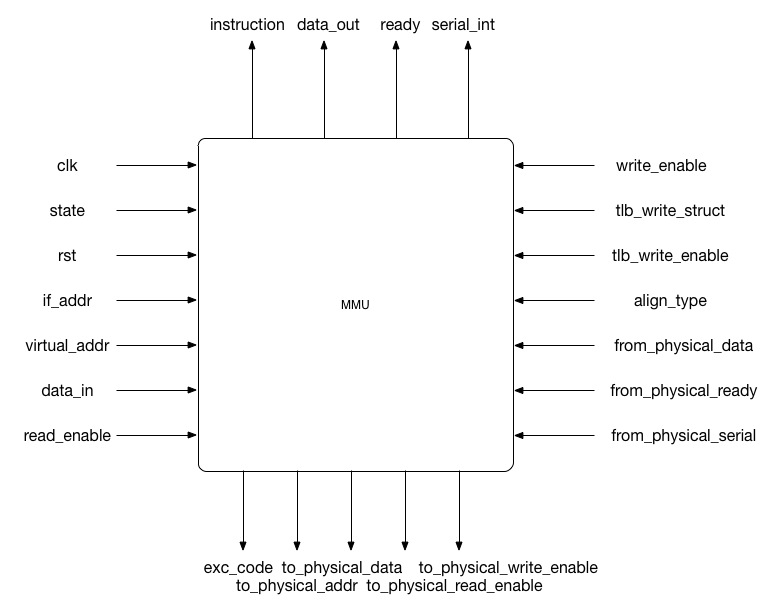
\includegraphics[width=0.9\textwidth]{chart/mmu.jpg}
            \end{figure}
        \subsubsection{内部实现}
            MMU模块作为真实访问物理内存阶段的预处理阶段,%
            完成对内存的读写控制,%
            完成TLB查询,充填TLB,抛出TLB异常等操作,%
            并且检查地址是否对齐,根据指令类型抛出地址不对齐异常。
            
            时钟控制:
            \begin{minipage}[t]{0.8\linewidth}
                访存阶段上升沿:%
                    虚拟地址到物理地址的转换,检查地址是否对齐%
                访存阶段下降沿:%
                    抛出TLB、地址不对齐等异常,%
                    将访存信号传递给物理内存,开始实际访存访问。%
            \end{minipage}
            
            读写控制:%
            \begin{minipage}[t]{0.8\linewidth}
                \begin{enumerate}
                \item
                    从MEM模块输入的读写使能信号需要经过处理后输出到物理访存模块%
                    访存条件为上层有使能信号,处于合适的CPU阶段%
                    地址转换不出现异常,物理访存处于停止状态%
                \item
                    如果当前state为取指令阶段,则一定为内存读取状态。%
                    如果当前为第一访存阶段,%
                        因为SB指令读写使能均为1,所以需要进行。%
                        如果mem\_read\_enable为1则进行读操作,%
                        否则如果mem\_write\_enable为1则进行写操作。%
                    如果当前为第二访存阶段,%
                        则一定为SB指令,进行写操作。%
                \end{enumerate}
            \end{minipage}
            
            地址映射:%
            \begin{minipage}[t]{0.8\linewidth}
                根据实际访问的地址值进行判断。%
                只对部分地址%
                ([0x20000000 $\sim$0x80000000]%
                和%
                [0xC0000000 $\sim$0xFFFFFFFF])% 
                进行映射,其他地址不经转换,直接访问。%
            \end{minipage}
            
            异常与中断:
            \begin{minipage}[t]{0.8\linewidth}
                MMU模块可能出现5种异常,一种中断%
                异常信号输出为exc\_code, %
                中断信号输出为serial\_int,输出到异常处理模块。%
                异常、中断信号产生时间为访存的时钟下降沿,%
                在下一个时钟下降沿就会被清空,%
                因此需要异常处理模块及时记录异常信息

                异常中断产生之后,物理内存访问的两个enable为全都会被强制置零,%
                保证在异常状态下不会产生实际的访存操作。

                \begin{enumerate}
                \item
                地址不对齐异常两种:%
                    根据指令类型判断当前指令是否需要对齐地址进行访问。%
                    (LB/SB/LBU指令不需要对齐地址,LHU指令对齐方式待定)%
                    根据访存地址后两位判断地址是否对齐。%
                    根据读写使能最终确定两种异常中的某一种。%
                \item
                TLB异常共三种:%
                    均在TLB查找结束之后生成。%
                    TLB缺失异常信号,根据查找的结果进行判断,%
                    如果为全零则根据度写使能触发异常。%
                    TLB修改异常,根据TLB查找结果的D标志位进行判断。%
                \item
                串口中断:%
                    直接将物理访存模块的中断信号输出,%
                    中断信号产生后将会一直保持,%
                    同时由于EXL位屏蔽中断,并不会产生实际的影响%
                    直到对串口进行读取操作之后,串口中断才消除。
                \end{enumerate}
            \end{minipage}
            
            TLB表查找:%
            \begin{minipage}[t]{0.8\linewidth}
                TLB表查找过程 %
                \begin{enumerate}
                \item
                    采用for\_generate/if\_generate语句生成TLB查找表。%
                    实际效果相当于将输入的虚拟地址高19位复制16份,%
                    同时与16个EntryHi进行比较,%
                    结果为16位std\_logic\_vector,其中只有1位为1,其余15位为0。%
                \item
                    再利用for\_generate/if\_generate语句生成TLB结果暂存表,%
                    为32*21矩阵%
                    32行对应一个16个TLB表项全部Lo部分,%
                    21为20位物理地址加一位D标志位。%
                \item
                    利用并行比较结果和虚拟地址最低位,%
                    共同对暂存表进行与操作,%
                    由于其中包含大量的0,%
                    最终只选择出1*21的std\_logic\_vector向量,%
                    即为20位物理地址与一位D标记位。%
                \item
                    如果查找到TLB查找到物理地址,%
                    且D标记位有效,则TLB查找成功,否则查找失败。%
                \end{enumerate}
            \end{minipage}

            TLB表重填:%
            \begin{minipage}[t]{0.8\linewidth}
                TLB表写入过程%
                \begin{enumerate}
                \item
                    TLB数据来源来自于CP0寄存器,%
                    共需要Index、PageMask、EntryHi、EntryLo0、EntryLo1%
                    五个寄存器的数值。%
                    CP0模块与MMU模块之间始终有以上5个寄存器的连线,%
                    始终能够获得CP0寄存器的最新值。%
                \item
                    TLB充填发生在TLBWI指令的执行阶段,%
                    在时钟上升沿、state为执行阶段、%
                    tlb\_enable使能信号为1的情况下,重填TLB表项。%
                \end{enumerate}
            \end{minipage}

    \subsection{CP0模块}
        \subsubsection{端口说明}
                    \begin{tabularx}{\textwidth}{lll}
            \toprule
            端口名          & 端口方向  & 端口类型 \\
            \cmidrule(l){2-3}
            &
            \multicolumn{2}{X}{端口描述} \\
            \midrule
            clk             & in        & std\_logic \\
            \cmidrule(l){2-3}
            &
            \multicolumn{2}{X}{
                CPU时钟信号
            } \\
            \midrule
            state           & in        & std\_logic\_vector(3 downto 0) \\
            \cmidrule(l){2-3}
            &
            \multicolumn{2}{X}{
                CPU当前状态
            } \\
            \midrule
	        normal\_cp0\_in & in        & std\_logic\_vector(37 downto 0) \\
            \cmidrule(l){2-3}
            &
            \multicolumn{2}{X}{
	            指令引发的CP0读写操作的输入,格式上,%
                37位为写使能,36-32位为地址,31-0位为数据。

	            读写均在时钟上升沿触发,%
                因此要求数据在时钟上升沿之前准备好。

	            状态方面,读操作发生在ID阶段的上升沿,%
                写操作发生在ALU阶段的上升沿。
            } \\
            \midrule
	        bad\_v\_addr\_in & in       & std\_logic\_vector(31 downto 0) \\
            \cmidrule(l){2-3}
            &
            \multicolumn{2}{X}{
	            异常发生时写入bad\_v\_addr\_in的数据,%
                要求数据在时钟上升沿之前准备好。%
                使能为interrupt\_start\_in。
            } \\
            \midrule
	        entry\_hi\_in   & in        & std\_logic\_vector(19 downto 0) \\
            \cmidrule(l){2-3}
            &
            \multicolumn{2}{X}{
	            异常发生时写入entry\_hi\_in高20位的数据,%
                要求数据在时钟上升沿之前准备好。%
                使能为interrupt\_start\_in。
            } \\
            \midrule
	        interrupt\_start\_in & in   & std\_logic \\
            \cmidrule(l){2-3}
            &
            \multicolumn{2}{X}{
	            异常写入的使能,控制异常数据的写入,%
                并将status(1)制1.
            } \\
            \midrule
	        cause\_in       & in        & std\_logic\_vector(4 downto 0) \\
            \cmidrule(l){2-3}
            &
            \multicolumn{2}{X}{
	            异常发生时写入cause的6-2位的数据,%
                要求数据在时钟上升沿之前准备好。%
                使能为interrupt\_start\_in。
            } \\
            \midrule
	        epc\_in         & in        & std\_logic\_vector(31 downto 0) \\
            \cmidrule(l){2-3}
            &
            \multicolumn{2}{X}{
	            异常发生时写入epc的数据,%
                要求数据在时钟上升沿之前准备好。%
                使能为interrupt\_start\_in。
            } \\
            \midrule
	        eret\_enable    & in        & std\_logic \\
            \cmidrule(l){2-3}
            &
            \multicolumn{2}{X}{
	            eret的使能信号,%
                将status(1)置0.优先于interrupt\_start\_in起效。

	            请注意,这一数据应当在ALU阶段上升沿之前准备好。
            } \\
            \midrule
	        cp0\_e          & in        & std\_logic \\
	        \cmidrule(l){2-3}
            &
            \multicolumn{2}{X}{
                CP0部分的使能信号。
            } \\
            \midrule
	        addr\_value     & out       & std\_logic\_vector(31 downto 0) \\
            \cmidrule(l){2-3}
            &
            \multicolumn{2}{X}{
	            normal\_cp0\_in读操作时读出的数据,%
                ID阶段上升沿之后起效,%
                下一ID阶段上升沿之前均不变。

	            初始值为全0.
            } \\
            \midrule
	        all\_regs       & out       & std\_logic\_vector(1023 downto 0) \\
            \cmidrule(l){2-3}
            &
            \multicolumn{2}{X}{
	            即时输出全部CP0寄存器的值,%
                CP0寄存器数值被修改的时间内不保证数值稳定。
            } \\
            \midrule
	        compare\_interrupt & out    & std\_logic \\
            \cmidrule(l){2-3}
            &
            \multicolumn{2}{X}{
	            clock寄存器与compare寄存器数值相同之后被置1;%
                修改compare寄存器的值后置0%
                且该周期不比较clock寄存器与compare寄存器的值。%
	            缺少将此值恢复为0的信号。%
	            变为1后,若不手动恢复为0或者修改compare寄存器,%
                则1保持。此输出值被检测到为1时触发中断,%
                任一上升沿均可检测,不需太早处理。
            } \\

            \bottomrule
        \end{tabularx}

            \begin{figure}[!hbp]
                \centering
                \caption{CP0模块端口示意图}
                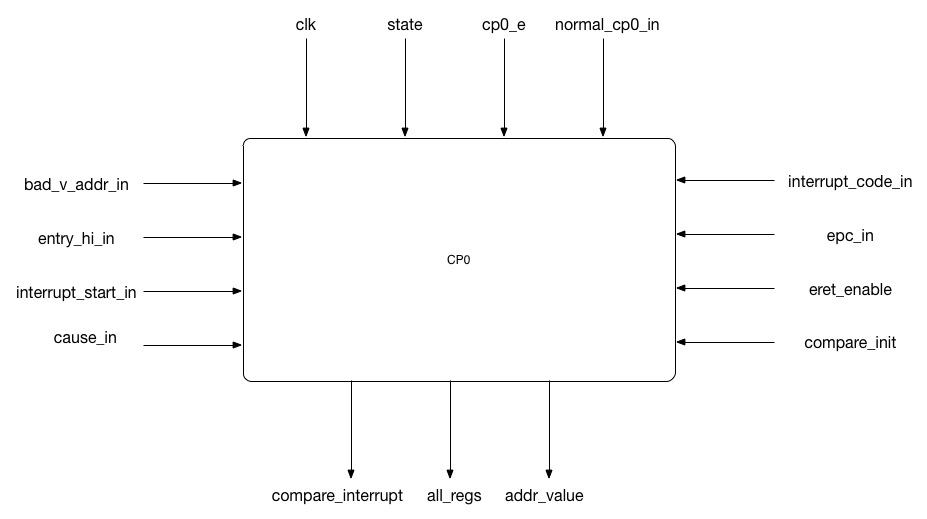
\includegraphics[width=0.9\textwidth]{chart/cp0.jpg}
            \end{figure}
        \subsubsection{内部实现}
            时钟触发。%
            检测到cp0\_e为0时,对内部值进行初始化。%
            否则,时钟上升沿时根据state进行相应操作。%
            若state为ID,根据输入地址进行读取操作。%
            若state为ALU,首先本次指令是否为ERET,%
            即检查eret\_enable,如果为1则将status(1)置0。%
            然后检测本次指令是否为写CP0,即检查normal\_cp0\_in(37),%
            如果需要写则进行CP0写入。注意,此时不进行clock的自增。%
            对于其他state,检查interrunp\_start\_in是否为1,%
            如果为1说明要进行异常信息的写入。%
            
            除此之外,还要进行clock寄存器与compare寄存器的比较,%
            compare寄存器的原有值被保存,如果修改,%
            则更新原有值,并将时钟中断置0;%
            否则,比较两寄存器的值,如果相等则置1,否则不变。%
            因此两寄存器第一次相等之后,触发时钟中断。%
            一定要注意,需要将时钟中断恢复的信号!

            CP0模块状态跳转:%
            无。%

            CP0模块异常触发:%
            任何时候检查到compre\_interrupt为1均触发异常。%
            此信号会保持且无需即时相应,在适应的时候触发异常即可。
    
    \subsection{异常处理模块}
        \subsubsection{端口说明}
                    \begin{tabularx}{\textwidth}{lll}
            \toprule
            端口名          & 端口方向  & 端口类型 \\
            \cmidrule(l){2-3}
            &
            \multicolumn{2}{X}{端口描述} \\
            \midrule
            clk             & in        & std\_logic \\
            \cmidrule(l){2-3}
            &
            \multicolumn{2}{X}{
                CPU时钟信号
            } \\
            \midrule
            state           & in        & status \\
            \cmidrule(l){2-3}
            &
            \multicolumn{2}{X}{
                自定义状态集合
            } \\
            \midrule
            exception\_e    & in        & std\_logic \\
            \cmidrule(l){2-3}
            &
            \multicolumn{2}{X}{
                exception模块使能信号
            } \\
            \midrule
            mmu\_exc\_code  & in        & std\_logic\_vector(2 downto 0) \\
            \cmidrule(l){2-3}
            &
            \multicolumn{2}{X}{
                来自MMU的异常信号,%
                表示TLB\_MODIFIED、TLB\_L、TLB\_S、ADE\_L、ADE\_S异常。%
                要求exception阶段时钟上升沿之前保持。
            } \\
            \midrule
            serial\_int     & in        & std\_logic \\
            \cmidrule(l){2-3}
            &
            \multicolumn{2}{X}{
                来自串口的异常信号。要求exception阶段时钟上升沿之前保持。
            } \\
            \midrule
            compare\_interrupt & in     & std\_logic \\
            \cmidrule(l){2-3}
            &
            \multicolumn{2}{X}{
                来自CP0的时钟中断信号。要求exception阶段时钟上升沿之前保持。
            } \\
            \midrule
            id\_exc\_code   & in        & std\_logic\_vetor(1 downto 0) \\
            \cmidrule(l){2-3}
            &
            \multicolumn{2}{X}{
                来自ID的异常信号,表示SYSCAL,RI异常。要求exception阶段时钟上升沿之前保持。
            } \\
            \midrule
            pc\_in          & in        & std\_logic\_vector(31 downto 0) \\
            \cmidrule(l){2-3}
            &
            \multicolumn{2}{X}{
                本指令的PC,来自CPU模块。要求exception阶段时钟上升沿之前保持。
            } \\
            \midrule
            v\_addr\_in     & in        & std\_logic\_vector(31 downto 0) \\
            \cmidrule(l){2-3}
            &
            \multicolumn{2}{X}{
                目前的访存虚拟地址,来自MMU。%
                要求exception阶段时钟上升沿之前保持。
            } \\
            \midrule
	        old\_entry\_hi  & in        & std\_logic\_vector(19 downto 0) \\
            \cmidrule(l){2-3}
            &
            \multicolumn{2}{X}{
                旧的entry\_hi,用于entry\_hi不变的情况,来自CP0。%
                要求exception阶段时钟上升沿之前保持。
            } \\
            \midrule
            old\_interrupt\_code & in   & std\_logic\_vector(5 downto 0) \\
            \cmidrule(l){2-3}
            &
            \multicolumn{2}{X}{
                旧的中断号,用于中断号不变的情况,来自CP0。%
                要求exception阶段时钟上升沿之前保持。
            } \\
            \midrule
            bad\_v\_addr\_out & out     & std\_logic\_vector(31 downto 0) \\
            \cmidrule(l){2-3}
            &
            \multicolumn{2}{X}{
                bad\_v\_addr输出值,交给CP0模块进行写入,可以保持到下次改变。
            } \\
            \midrule
            entry\_hi\_out  & out       & std\_logic\_vector(19 downto 0) \\
            \cmidrule(l){2-3}
            &
            \multicolumn{2}{X}{
                entry\_hi输出值,交给CP0模块进行写入,可以保持到下次改变。
            } \\
            \midrule
	        interrupt\_start\_out & out & std\_logic \\
            \cmidrule(l){2-3}
            &
            \multicolumn{2}{X}{
                CP0模块的异常写入使能,%
                控制CP0模块开始写入异常信息,%
                可以保持到下一时钟上升沿之前。
            } \\
            \midrule
	        cause\_out      & out       & std\_logic\_vector(4 downto 0) \\
            \cmidrule(l){2-3}
            &
            \multicolumn{2}{X}{
                异常号输出值,交给CP0模块进行写入,可以保持到下次改变。
            } \\
            \midrule
	        interrupt\_cause\_out & out & std\_logic\_vector(5 downto 0) \\
            \cmidrule(l){2-3}
            &
            \multicolumn{2}{X}{
                中断号输出值,交给CP0模块进行写入,可以保持到下次改变。
            } \\
            \midrule
	        epc\_out        & out       & std\_logic\_vector(31 downto 0) \\
            \cmidrule(l){2-3}
            &
            \multicolumn{2}{X}{
                EPC输出值,交给CP0模块进行写入,可以保持到下次改变
            } \\
            \midrule
	        pc\_sel0        & out       & std\_logic \\
            \cmidrule(l){2-3}
            &
            \multicolumn{2}{X}{
                IF阶段选择PC的pc\_sel的0位,%
                若为1表示应选择异常处理向量作为新的PC。%
                可以保持到下一时钟上升沿之前。
            } \\

            \bottomrule
        \end{tabularx}



            \begin{figure}[!hbp]
                \centering
                \caption{异常处理模块端口示意图}
                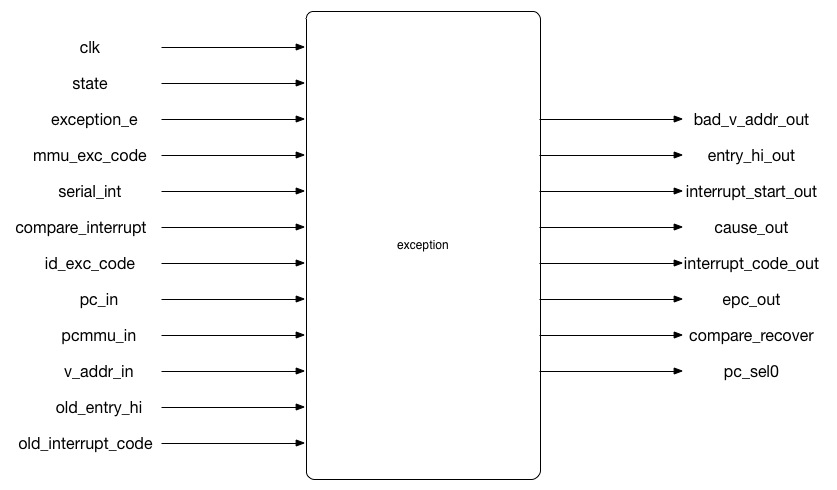
\includegraphics[width=0.9\textwidth]{chart/exception.jpg}
            \end{figure}
        \subsubsection{内部实现}

	        exception负责产生、发送异常信息,%
            根据目前的异常号、中断号,%
            从输入值选择适当的异常信息作为写入CP0的数据。%
	        
            除写入异常信息外,%
            还需将interrupt\_start\_out,pc\_sel0两个控制信号置1,%
            使CP0准备写入以及异常信息保存后跳转到EBase。%
            其他情况下将其置0。

            异常处理设计简述:
            \begin{enumerate}
            \item
	        需要考虑的异常:
                \begin{enumerate}
                    \item
                    Interrupt,外部中断。包括时钟中断,串口中断。
                    \item
                    TLB Modify,对内存的只读部分进行写操作。
                    \item
                    TLBL,读时发生的TLB miss
                    \item
                    TLBS,写时发生的TLB miss
                    \item
                    ADEL,对非对齐地址进行读操作
                    \item
                    ADES,对非对齐地址进行写操作
                    \item
                    SYSCALL,系统调用
                    \item
                    RI,执行未定义指令
                \end{enumerate}
            \item
            对于以下异常,不予考虑:
                \begin{enumerate}
                    \item
                    访问未定义的CP0寄存器。未定义的寄存器视作通用寄存器。
                    \item
                    运算溢出。不予处理。
                \end{enumerate}
            \item
            异常处理数据来源(部分异常中未明确提到的信号,请保持原值):
                \begin{enumerate}
                    \item
                    Interrupt:
                        由CP0的compare信号与串口的可读信号触发,%
                        在IF阶段开始时检查。
                        异常被处理前信号一直保持,%
                        时钟中断被处理后需给CP0模块控制信号消除异常,%
                        串口中断被处理后由串口读写部分消除异常。
                        CP0 status(EXL)即(13)(1)位为'1'时,%
                        表示处于异常处理中,不触发外部异常。
                        检查到异常时,记录异常号、中断号,%
                        bad\_v\_addr取当前指令的地址,EPC取当前指令的地址。
                    \item
                    TLB Modify:
                        由MMU的对应信号触发,发生在MEM阶段,在ID、WB阶段开始时检查。
                        异常在下一时钟下降沿消除,因此需在要求的上升沿进行检查。
                        检查到异常时,记录异常号,%
                        bad\_v\_addr取MMU提供的虚拟地址,%
                        EPC取当前指令的地址。
                    \item
                    TLBL:
                        由MMU的对应信号触发,发生在IF阶段或MEM阶段,%
                        在ID、WB阶段开始时检查。%
                        异常在下一时钟下降沿消除,%
                        因此需在要求的上升沿进行检查。%
                        检查到异常时,记录异常号,%
                        bad\_v\_addr取MMU提供的虚拟地址,%
                        EPC取当前指令的地址,EntryHi高20位取MMU提供虚拟地址。
                    \item
                    TLBS:
                        由MMU的对应信号触发,发生在MEM阶段,%
                        在ID、WB阶段开始时检查。
                        异常在下一时钟下降沿消除,%
                        因此需在要求的上升沿进行检查。%
                        检查到异常时,记录异常号,%
                        bad\_v\_addr取MMU提供的虚拟地址,EPC取当前指令的地址,%
                        EntryHi高20位取MMU提供虚拟地址。
                    \item
                    ADEL:
                        由MMU的对应信号触发,发生在IF阶段或MEM阶段,%
                        在ID、WB阶段开始时检查。%
                        异常在下一时钟下降沿消除,%
                        因此需在要求的上升沿进行检查。%
                        检查到异常时,记录异常号,%
                        bad\_v\_addr取MMU提供的物理地址,EPC取当前指令的地址。
                    \item
                    ADES:
                        由MMU的对应信号触发,发生在MEM阶段,%
                        在ID、WB阶段开始时检查。%
                        异常在下一时钟下降沿消除,%
                        因此需在要求的上升沿进行检查。%
                        检查到异常时,记录异常号,%
                        bad\_v\_addr取MMU提供的物理地址,EPC取当前指令的地址。
                    \item
                    SYSCALL:
                        由ID模块的对应信号触发,%
                        发生在ID阶段,在ALU阶段开始时检查。%
                        异常在下一时钟上升沿消除,%
                        因此需在要求的上升沿进行检查。%
                        检查到异常时,记录异常号,%
                        bad\_v\_addr取当前指令地址,EPC取当前指令的地址。
                    \item
                    RI:
                        由ID模块的对应信号触发,发生在ID阶段,%
                        在ALU阶段开始时检查。%
                        异常在下一时钟上升沿消除,%
                        因此需在要求的上升沿进行检查。%
                        检查到异常时,记录异常号,%
                        bad\_v\_addr取当前指令地址,EPC取当前指令的地址。
                \end{enumerate}
                \end{enumerate}

                exception模块状态跳转:
                    请无条件跳转至IF阶段。

                exception模块异常触发:
                    无。
